\section{Additional results}
\label{app:tables}

This appendix gives the per-cell switch rates behind \S\ref{sec:results-h1}
(Table~\ref{tab:switch-cells}), the H3 prediction table (Table~\ref{tab:h3}), and the per-stratum decision effects referred to in
\S\ref{sec:discussion} (Table~\ref{tab:strata}). It also shows the replication of the primary and
mention contrasts across all splits (Figure~\ref{fig:replication}, summarized in \S\ref{sec:results-h2}),
the gate results of every model attempted (Table~\ref{tab:models-gate}), the tracked-history
analysis per model (Table~\ref{tab:joint-by-model}), and Qwen3-14B's construction effects
(Figure~\ref{fig:constructions-14b}). Rows are ordered with routing, the task competent on the confirmation data, first.

\begin{table}[h]
\centering
\small
\setlength{\tabcolsep}{3pt}
\begin{tabular}{@{}lcccc@{}}
\toprule
Cell & Superseded & Other attr. & Mention & Unattached \\
\midrule
routing seq.  & 0.164 & 0.062 & 0.352 & 0.055 \\
routing int.  & 0.227 & 0.078 & 0.273 & 0.055 \\
routing comp. & 0.164 & 0.055 & 0.258 & 0.008 \\
\midrule
access seq.   & 0.133 & 0.070 & 0.148 & 0.094 \\
access int.   & 0.273 & 0.234 & 0.219 & 0.094 \\
access comp.  & 0.094 & 0.109 & 0.219 & 0.000 \\
\bottomrule
\end{tabular}
\caption{Net switch rate toward the wrong action, per cell and construction (confirmation, $n = 128$
histories per cell). Intervals are in the released analysis.}
\label{tab:switch-cells}
\end{table}

\begin{table}[h]
\centering
\small
\setlength{\tabcolsep}{3pt}
\begin{tabular}{@{}llcc@{}}
\toprule
Stratum & Vocab. & $D_{\mathrm{superseded}}$ & $\Delta_{\mathrm{mention}}$ \\
\midrule
routing seq.  & natural & 3.66 & $-2.32$ \\
routing int.  & natural & 4.03 & $-1.00$ \\
routing comp. & natural & 3.07 & $-2.38$ \\
routing seq.  & opaque  & 2.53 & $-2.17$ \\
routing int.  & opaque  & 2.78 & $-1.32$ \\
routing comp. & opaque  & 2.73 & $-0.87$ \\
\midrule
access seq.   & natural & 3.61 & $-1.16$ \\
access int.   & natural & 4.01 & $-0.06$ \\
access comp.  & natural & 3.65 & $-2.21$ \\
access seq.   & opaque  & 4.53 & $-1.10$ \\
access int.   & opaque  & 4.43 & $-1.42$ \\
access comp.  & opaque  & 3.20 & $-1.72$ \\
\bottomrule
\end{tabular}
\caption{Decision effects (nats) by task, cell and vocabulary (confirmation, 64 histories per stratum).
All $D_{\mathrm{superseded}}$ intervals exclude zero. The $\Delta_{\mathrm{mention}}$ interval includes zero
only for access, interleaved, natural ($[-1.01, 0.96]$).}
\label{tab:strata}
\end{table}

\paragraph{Replication across splits.} Four earlier, non-confirmatory splits of the same protocol family
(development and gate of the first redesign and of the confirmed protocol, on the standard template) show
which conclusions depend on wording (Figure~\ref{fig:replication}). $D_{\mathrm{superseded}}$ was
positive in all ten split-by-task estimates (3.133 to 6.599 nats), and $\Delta_{\mathrm{semantic}}$ in
nine of ten. $\Delta_{\mathrm{mention}}$ never favored the superseded assignment. On the standard template,
however, it ranged from $-0.806$ to $+0.163$, with six of eight intervals including zero. The size of the
mention advantage depends on wording.

\paragraph{Gate-rule estimates.} The replication amendment defined competent cells by each model\textquoteright s frozen gate. Table~\ref{tab:cross-model} uses the cells competent on the confirmation data, the rule used throughout the text. For Qwen3-8B, the gate rule instead selects routing int.+seq. ($n=256$): $D_{\mathrm{superseded}}=+3.248$, $\Delta_{\mathrm{semantic}}=+1.330$, $\Delta_{\mathrm{mention}}=-1.702$, net switch rate $+0.195$; access int. ($n=128$): $D_{\mathrm{superseded}}=+4.221$, $\Delta_{\mathrm{semantic}}=-0.132$, $\Delta_{\mathrm{mention}}=-0.740$, net switch rate $+0.273$. For Qwen3-14B, the gate rule selects the same cells.


\begin{figure*}[t]
\centering
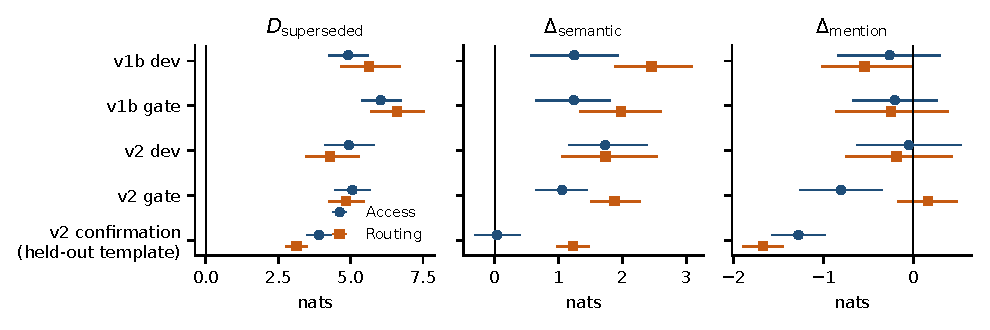
\includegraphics[width=\textwidth]{figures/replication.pdf}
\caption{Primary and mention contrasts across all five splits run under the v1b and v2 protocols (95\%
intervals for development and gate splits, 97.5\% for the confirmation's primary contrasts and 95\% for
its $\Delta_{\mathrm{mention}}$). Development and gate splits used the standard template, and v1b also kept
the \lit{Answer:} line. Only the confirmation is confirmatory.}
\label{fig:replication}
\end{figure*}

\begin{table}[h]
\centering
\small
\setlength{\tabcolsep}{3pt}
\resizebox{\columnwidth}{!}{%
\begin{tabular}{@{}lccc@{}}
\toprule
& Overall & Access & Routing \\
\midrule
Failures & 892/6144 & 454/3072 & 438/3072 \\
Log loss, prevalence & 0.414 & 0.419 & 0.410 \\
Log loss, pre-decision & 0.346 & 0.323 & 0.358 \\
AUROC, pre-decision & 0.780 & 0.834 & 0.729 \\
AUROC, $+R_{\mathrm{easy}}$ & 0.779 & 0.833 & 0.730 \\
Gain from $R_{\mathrm{easy}}$ & $+0.0004$ & $-0.0006$ & $+0.0013$ \\
\bottomrule
\end{tabular}}
\caption{H3: out-of-fold prediction of strict downstream failure on historical-construction items
(history-grouped five-fold cross-validation). 95\% intervals for the gain: overall $[-0.0011, 0.0019]$,
access $[-0.0020, 0.0008]$, routing $[-0.0022, 0.0047]$. The decision's own action confidence, a contemporaneous
reference that is not available before the decision, reaches AUROC 1.000.}
\label{tab:h3}
\end{table}

\begin{table}[h]
\centering
\small
\setlength{\tabcolsep}{3pt}
\begin{tabular}{@{}llcccc@{}}
\toprule
Model & Cell & Direct & No hist. & History & Comp. \\
\midrule
Qwen3-8B & routing seq. & 0.977 & 0.938 & 0.779 & yes \\
 & routing int. & 0.986 & 0.938 & 0.779 & yes \\
 & routing comp. & 0.945 & 0.938 & 0.752 & no \\
 & access seq. & 0.889 & 0.906 & 0.822 & no \\
 & access int. & 0.953 & 0.938 & 0.877 & yes \\
 & access comp. & 0.953 & 0.859 & 0.883 & no \\
\midrule
Qwen3-14B & routing seq. & 0.996 & 0.922 & 0.854 & yes \\
 & routing int. & 1.000 & 1.000 & 0.846 & yes \\
 & routing comp. & 0.997 & 1.000 & 0.814 & yes \\
 & access seq. & 0.991 & 0.781 & 0.729 & no \\
 & access int. & 0.977 & 0.828 & 0.748 & no \\
 & access comp. & 0.946 & 0.828 & 0.697 & no \\
\midrule
Gemma 3 4B & routing seq. & 0.939 & 0.688 & 0.645 & no \\
 & routing int. & 0.964 & 0.609 & 0.488 & no \\
 & routing comp. & 0.916 & 0.625 & 0.533 & no \\
 & access seq. & 0.945 & 0.719 & 0.678 & no \\
 & access int. & 0.936 & 0.609 & 0.676 & no \\
 & access comp. & 0.946 & 0.672 & 0.641 & no \\
\bottomrule
\end{tabular}
\caption{Frozen gate split (384 histories, identical rows for every model): strict direct current-state retrieval, current-only decision accuracy, decision accuracy with history, and whether the cell is competent (direct $\ge 0.95$, no history $\ge 0.90$, invalid $\le 0.05$). This gate decided eligibility to generate confirmation data. Labels computed on the confirmation data (Table~\ref{tab:competence}, Table~\ref{tab:cross-model}) can differ: Qwen3-8B access int. is competent here and not competent on the confirmation data; Qwen3-8B routing comp. is not competent here and competent on the confirmation data.}
\label{tab:models-gate}
\end{table}


\begin{table}[h]
\centering
\small
\setlength{\tabcolsep}{3pt}
\begin{tabular}{@{}llccc@{}}
\toprule
Model & Construction & Kept & Net switch rate & Switched \\
\midrule
Qwen3-8B & superseded & 348/384 & $+0.158$ {\scriptsize $[+0.118, +0.198]$} & 58 / 3 \\
 & other attr. & 357/384 & $+0.048$ {\scriptsize $[+0.014, +0.084]$} & 29 / 12 \\
 & mention & 349/384 & $+0.278$ {\scriptsize $[+0.232, +0.327]$} & 97 / 0 \\
 & unattached & 351/384 & $+0.034$ {\scriptsize $[+0.009, +0.060]$} & 17 / 5 \\
\midrule
Qwen3-14B & superseded & 376/384 & $+0.165$ {\scriptsize $[+0.128, +0.205]$} & 65 / 3 \\
 & other attr. & 367/384 & $+0.136$ {\scriptsize $[+0.101, +0.174]$} & 52 / 2 \\
 & mention & 363/384 & $+0.168$ {\scriptsize $[+0.132, +0.207]$} & 61 / 0 \\
 & unattached & 375/384 & $+0.024$ {\scriptsize $[+0.000, +0.051]$} & 16 / 7 \\
\bottomrule
\end{tabular}
\caption{Routing histories the model demonstrably tracks (criteria of Table~\ref{tab:joint}), per model and construction. Condition (ii), initial-state retrieval, is asked only on the superseded members and is applied at the history level to all four constructions. Net switch rate with 95\% history-bootstrap intervals; switched: histories switched to the wrong / to the correct action.}
\label{tab:joint-by-model}
\end{table}


\begin{figure*}[t]
\centering
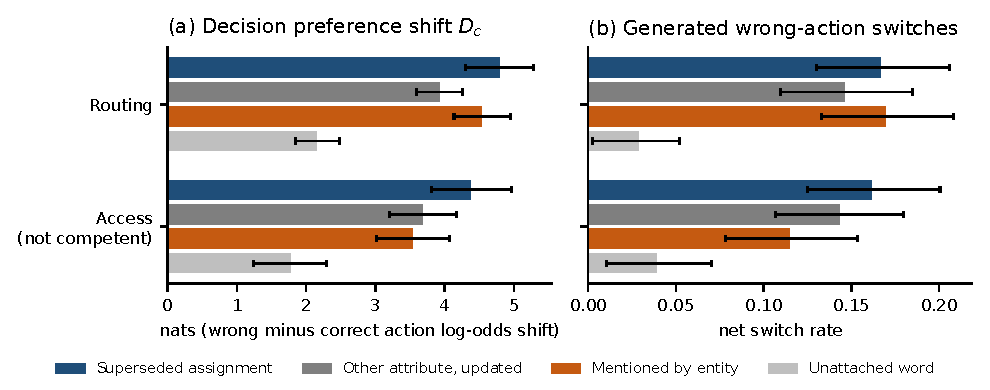
\includegraphics[width=\textwidth]{figures/constructions_qwen3_14b.pdf}
\caption{Qwen3-14B: decision effects by construction (confirmation, 384 histories per task, 95\%
history-bootstrap intervals), as in Figure~\ref{fig:constructions}. Routing cells meet the competence criteria on the confirmation data; access cells do not.}
\label{fig:constructions-14b}
\end{figure*}
